\documentclass[11pt]{article}

\usepackage{amsfonts}
%\usepackage{geometry}
\usepackage[paper=a4paper, 
            left=20.0mm, right=20.0mm, 
            top=25.0mm, bottom=25.0mm]{geometry}
\pagestyle{empty}
\usepackage{graphicx}
\usepackage{fancyhdr, lastpage, bbding, pmboxdraw}
\usepackage[usenames,dvipsnames]{color}
\definecolor{darkblue}{rgb}{0,0,.6}
\definecolor{darkred}{rgb}{.7,0,0}
\definecolor{darkgreen}{rgb}{0,.6,0}
\definecolor{red}{rgb}{.98,0,0}
\usepackage[colorlinks,pagebackref,pdfusetitle,urlcolor=darkblue,citecolor=darkblue,linkcolor=darkred,bookmarksnumbered,plainpages=false]{hyperref}
\renewcommand{\thefootnote}{\fnsymbol{footnote}}

\pagestyle{fancyplain}
\fancyhf{}
\lhead{ \fancyplain{}{Course Name} }
%\chead{ \fancyplain{}{} }
\rhead{ \fancyplain{}{\today} }
%\rfoot{\fancyplain{}{page \thepage\ of \pageref{LastPage}}}
\fancyfoot[RO, LE] {Page \thepage\ of \textcolor{black}{\pageref{LastPage}} }
\thispagestyle{plain}

%%%%%%%%%%%% LISTING %%%
\usepackage{listings}
\usepackage{caption}
\usepackage{subcaption}
\DeclareCaptionFont{white}{\color{white}}
\DeclareCaptionFormat{listing}{\colorbox{gray}{\parbox{\textwidth}{#1#2#3}}}
\captionsetup[lstlisting]{format=listing,labelfont=white,textfont=white}
\usepackage{verbatim} % used to display code
\usepackage{fancyvrb}
\usepackage{acronym}
\usepackage{amsthm, amsmath}
\usepackage{tikz}
    \usetikzlibrary{calc, arrows, arrows.meta, positioning}
\usepackage{amssymb,amsmath,stackengine}
\stackMath
\usepackage{ifthen}

\VerbatimFootnotes % Required, otherwise verbatim does not work in footnotes!

\definecolor{OliveGreen}{cmyk}{0.64,0,0.95,0.40}
\definecolor{CadetBlue}{cmyk}{0.62,0.57,0.23,0}
\definecolor{lightlightgray}{gray}{0.93}

\lstset{
	%language=bash,                          % Code langugage
	basicstyle=\ttfamily,                   % Code font, Examples: \footnotesize, \ttfamily
	keywordstyle=\color{OliveGreen},        % Keywords font ('*' = uppercase)
	commentstyle=\color{gray},              % Comments font
	numbers=left,                           % Line nums position
	numberstyle=\tiny,                      % Line-numbers fonts
	stepnumber=1,                           % Step between two line-numbers
	numbersep=5pt,                          % How far are line-numbers from code
	backgroundcolor=\color{lightlightgray}, % Choose background color
	frame=none,                             % A frame around the code
	tabsize=2,                              % Default tab size
	captionpos=t,                           % Caption-position = bottom
	breaklines=true,                        % Automatic line breaking?
	breakatwhitespace=false,                % Automatic breaks only at whitespace?
	showspaces=false,                       % Dont make spaces visible
	showtabs=false,                         % Dont make tabls visible
	columns=flexible,                       % Column format
	morekeywords={__global__, __device__},  % CUDA specific keywords
}

\newcommand{\question}[1]{\section*{\normalsize #1}}
% \newcommand{\mat}[1]{\begin{bmatrix}#1\end{bmatrix}}
% \newcommand{\extraspace}[]{
%     \begin{center}
%         \textbf{Use this page for extra space.}
%     \end{center}
% }


\DeclareMathOperator*{\argmax}{arg\,max}
\DeclareMathOperator*{\argmin}{arg\,min}
%\DeclareMathOperator*{\vec}[1]{\textbf{#1}}

\newcommand{\squig}{{\scriptstyle\sim\mkern-3.9mu}}
\newcommand{\lsquigend}{{\scriptstyle\lhd\mkern-3mu}}
\newcommand{\rsquigend}{{\scriptstyle\rule{.1ex}{0ex}\rhd}}
\newcounter{sqindex}
\newcommand\squigs[1]{%
  \setcounter{sqindex}{0}%
  \whiledo {\value{sqindex}< #1}{\addtocounter{sqindex}{1}\squig}%
}
\newcommand\rsquigarrow[2]{%
  \mathbin{\stackon[2pt]{\squigs{#2}\rsquigend}{\scriptscriptstyle\text{#1\,}}}%
}
\newcommand\lsquigarrow[2]{%
  \mathbin{\stackon[2pt]{\lsquigend\squigs{#2}}{\scriptscriptstyle\text{\,#1}}}%
}


\begin{document}
\begin{center}
    {\Large \{Written Assignment 1}}
\end{center}
\begin{center}
    Due: Friday 09/19/2025 @ 11:59pm EST
\end{center}

\section*{\textbf{Disclaimer}}
I encourage you to work together, I am a firm believer that we are at our best (and learn better) when we communicate with our peers. Perspective is incredibly important when it comes to solving problems, and sometimes it takes talking to other humans (or rubber ducks in the case of programmers) to gain a perspective we normally would not be able to achieve on our own. The only thing I ask is that you report who you work with: this is \textbf{not} to punish anyone, but instead will help me figure out what topics I need to spend extra time on/who to help. When you turn in your solutions (please use some form of typesetting: do \textbf{NOT} turn in handwritten solutions), please note who you worked with at the very beginning of the pdf.\newline












\question{Question 1: Shortest Path Composition (10 points)}
Consider a graph $G = (V, E, w: E\rightarrow \mathbb{R}^{> 0})$ where $V$ is a set of vertices, $E$ is a set of (directed) edges, and $w$ is a \textit{weight function} that maps edges to weights where each weight is $> 0$. Let us define a path $p$ to be a sequence of edges where the destination vertex of one edge is the source vertex of the next edge (if the next edge exists). Let us define the \textit{cost} of an path the traditional way, i.e. the cost of a path $p$ is the sum of the edge weights in $p$:
$$cost(p) = \sum\limits_{e\in p} w(e)$$
Show that if we know a shortest path $p^* = a\rsquigarrow{x}{4}b$ from vertex $a$ to vertex $b$ has cost $x$. If we know $p^*$ passes through intermediary vertex $c$, then let $p_1 = a\rsquigarrow{y}{4}c$, and let $p_2 = c\rsquigarrow{z}{4}b$. Show that if $p^* = p_1 \cup p_2$, then $p_1$ is a shortest path from $a$ to $c$, and that $p_2$ is a shortest path from $c$ to $b$.\newline

\noindent\textbf{Note:} this is a \textbf{proof} question, meaning you must follow formal proof structure (see the examples on piazza for guidance).\newpage















\question{Question 2: Iterative Deepening (10 points)}
Consider an unweighted (e.g. a constant positive weighted) graph $G = (V, E)$ where $V$ is a set of vertices and $E$ is a set of (directed) edges. Recall that the expansion of all simple paths in a graph forms a tree, which is then expanded via a graph traversal algorithm. Recall that the way DFS traverses this expansion tree is by drilling down a path until it reaches a leaf vertex, then backing off to the parent and trying another branch. Also recall that \textit{Depth-Limited} DFS (DLDFS) is just like the normal DFS algorithm except it is configured via a hyperparameter called the ``depth'' of the search. This value (a positive integer) provides an upper bound on the number of edges a path can be expanded before DFS arbitrarily backs off (regardless of whether the current vertex is a leaf or not).\newline

\noindent The \textit{Iterative Deepening} algorithm is a single-source shortest-path algorithm that uses DLDFS as a subroutine. Iterative Deepening repeatedly calls DLDFS where each call is given a different depth limit: the first call to DLDFS uses a depth limit of 1, the second call to DLDFS uses a depth limit of 2, the third call to DLDFS uses a depth limit of 3, etc. Iterative Deepening continues to call DLDFS until a path to all vertices have been found (from the source vertex), or until it is determined any unreached vertices are no-longer reachable from the source node. Prove that when Iterative Deepening returns a path from the source to any other vertex, that this path is the shortest path between that pair of vertices.\newline

\noindent\textbf{Note:} this is a \textbf{proof} question, meaning you must follow formal proof structure (see the examples on piazza for guidance).\newpage











\question{Question 3: Graph Diameters and the Longest-Shortest Path (10 points)}
The diameter of an undirected, unweighted graph $G=(V, E)$ is defined to be the solution to the following optimization problem:
$$d = \max\limits_{\substack{(u,v)\in V \\ u\neq v}} \min\limits_{k\in\mathbb{Z}^{\ge 0}} cost(u\rsquigarrow{k}{4}v)$$
which in english is ``the largest of all the shortest paths in $G$'' where $u\rsquigarrow{k}{4}v$ is a path from vertex $u$ to vertex $v$ using exactly $k$ edges, and the cost of a path is the sum of the edge weights used in that path (in our case $cost(u\rsquigarrow{k}{4}v) = k$). Prove that the diameter of any unweighted, undirected graph is at most $|V|$ (the number of vertices in the graph).\newline

\noindent\textbf{Note:} this is a \textbf{proof} question, meaning you must follow formal proof structure (see the examples on piazza for guidance).\newpage











\question{Question 4: Dijkstras Algorithm and Shortest Paths (20 points)}
Consider a graph $G = (V, E, w: E\rightarrow \mathbb{R}^{> 0})$ where $V$ is a set of vertices, $E$ is a set of (directed) edges, and $w$ is a \textit{weight function} that maps edges to weights where each weight is $> 0$. If we were to search for the shortest path between a pair of vertices in such a graph, we would be forced to use dijkstras algorithm as BFS and Iterative Deepening assume a constant weighting. Prove that when dijkstras algorithm returns a path from the source to any other vertex, that this path is the shortest path between that pair of vertices.\newline

\noindent\textbf{Note:} this is a \textbf{proof} question, meaning you must follow formal proof structure (see the examples on piazza for guidance).\newpage










\question{Extra Credit: Shortest Path in a Lattice Graph (50 points)}
Let $G = (V, E)$ be a directed graph defined on a $n\times n$ lattice (see Figure~\ref{fig:lattice}). The vertices of $G$ are the nodes of the lattice and the edges of $G$ connect the nodes of the lattice as shown in Figure~\ref{fig:lattice}. Therefore, $G$ has $O(n^2)$ vertices and $O(n^2)$ edges. All of the edges in $G$ have weight 0 and all of the vertices in $G$ have weights that are arbitrarily positive real numbers. The length of any path in $G$ is defined as the sum of the weights of all the vertices used in the path. Assume that you are already given an algorithm $ALG(G', s,t)$ for computing a shortest path and its length between any two specified vertices $s$ and $t$ in an arbitrary portion $G'$ of the lattice graph $G$ in $O(|V'| + |E'|)$ where $V'$ is the set of vertices in $G'$ and $E'$ is the set of edges in $G'$. Design and prove your most efficient algorithm (by making using of $ALG(G', s,t)$ in any way you like) for computing a path $P^*$ which has the minimum length amongst the shortest paths from vertices $v_{1, i}\rightarrow v_{n,i}$ where $i=1,2,\cdots,n$. In english, we would say that if we were to find the shortest path from $v_{1,1}\rightarrow v_{n,1}$, then find the shortest path from $v_{1,2}\rightarrow v_{n,2}$, then $v_{1,3}\rightarrow v_{n,3}$, etc., the shorest path $P^*$ would be the shortest of these shortest paths.
\begin{figure}[!h]
    \centering
    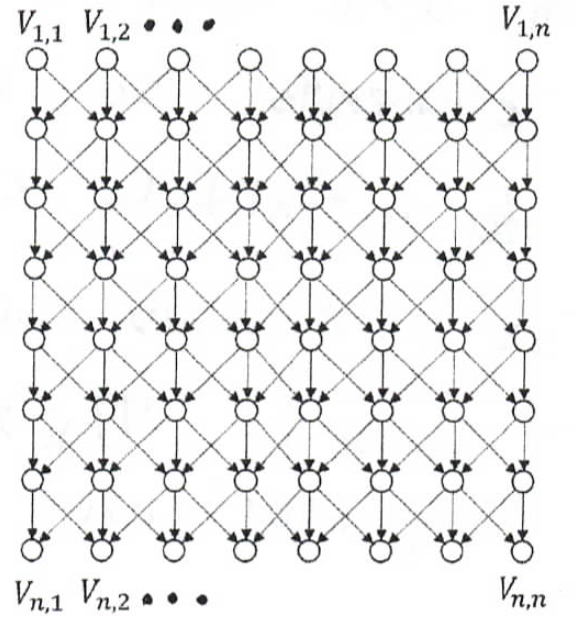
\includegraphics[width=0.5\linewidth]{./imgs/lattice.png}
    \caption{A directed graph $G$ defined on a $n\times n$ lattice.}
    \label{fig:lattice}
\end{figure}


\end{document}

